% 导入必要的包
\usepackage{tikz} % 用于程序化创建图形
\usepackage{calc} % 在 LaTeX 中进行计算
\usepackage{booktabs} % 创建专业的表格

% 定义自定义颜色
\definecolor{color1}{HTML}{000060} % 深蓝色
%\definecolor{color1}{HTML}{8C260F} % 注释掉的备用深红色
\definecolor{color2}{HTML}{333333} % 深灰色

% 使用 fontspec 包设置字体
\usepackage{fontspec}
\defaultfontfeatures{Mapping=tex-text} % 特殊字符映射
\setmainfont % 主字体设置
[BoldFont=Lato-Bold.ttf, % 粗体字体
ItalicFont=Lato-Italic.ttf, % 斜体字体
BoldItalicFont=Lato-BoldItalic.ttf] % 粗斜体字体
{Lato-Regular.ttf} % 正文字体
\newfontfamily\headingfont[ItalicFont=Lato-BlackItalic.ttf]{Lato-Black.ttf} % 标题字体

% 页面布局设置
\usepackage{geometry}
\geometry{a4paper, % A4 纸张
	hmargin=20mm,vmargin=20mm, % 页边距设置
	head=0ex,foot=0ex} % 页眉和页脚

\linespread{1.3} % 行距设置

% 设置标题和标题格式
\usepackage[hang]{caption}
\DeclareCaptionFormat{upper}{#1#2\uppercase{#3}\par} % 设置标题格式为大写
\captionsetup{labelfont={bf,color=color2},textfont={normalsize,color=color2},format = upper,figurename=图,tablename=表}

% 自定义章节格式
\usepackage{titlesec}
%\titleformat{\chapter}{\headingfont\LARGE\bfseries\scshape\color{color1}}{\thechapter}{1em}{}[\titlerule]
\titleformat{\section}{\color{color1}\headingfont\Large\bfseries\uppercase}{\thesection}{1em}{}[\titlerule]
\titleformat{\subsection}{\color{color1}\headingfont\large\bfseries\uppercase}{\thesubsection}{1em}{}
\titleformat{\subsubsection}{\color{color1}\headingfont\bfseries\uppercase}{\thesubsubsection}{1em}{}

% 设置页眉和页脚
\usepackage{fancyhdr}
\pagestyle{fancy}
\lhead{} % 左页眉
\chead{} % 中间页眉
\makeatletter
\rhead{\color{color2}\@date} % 右页眉显示日期
\makeatother
\newlength{\myheight}
\lfoot{
	\settoheight{\myheight}{\thepage}
	\raisebox{-3ex-0.5\myheight}{
\includegraphics[height=4ex]{logo.png}} % 左页脚显示 logo 图片
}
\cfoot{\color{color2}} % 中间页脚
\rfoot{\color{color2}\thepage} % 右页脚显示页码
\renewcommand\headrulewidth{0pt} % 去掉页眉下的横线
\renewcommand\footrulewidth{0pt} % 去掉页脚上的横线

% 自定义封面
\makeatletter
\newcommand*\DefVar[1]{\@namedef{#1}##1{\global\@namedef{get#1}{##1}}}
\DefVar{summary}
\renewcommand{\maketitle}{
	\vfill 
	\begin{center}
		% 插入标题
		
\begin{tikzpicture}
			\node[draw=none, fill=color1, inner sep=10pt, text width=\textwidth-20pt, text centered] {\color{white}\headingfont\bfseries\huge\@title};
		\end{tikzpicture}
		
		% 去除标题和图片之间的缝隙
		\vspace{-2mm}
		
		% 插入封面图片,并调整其位置和大小
		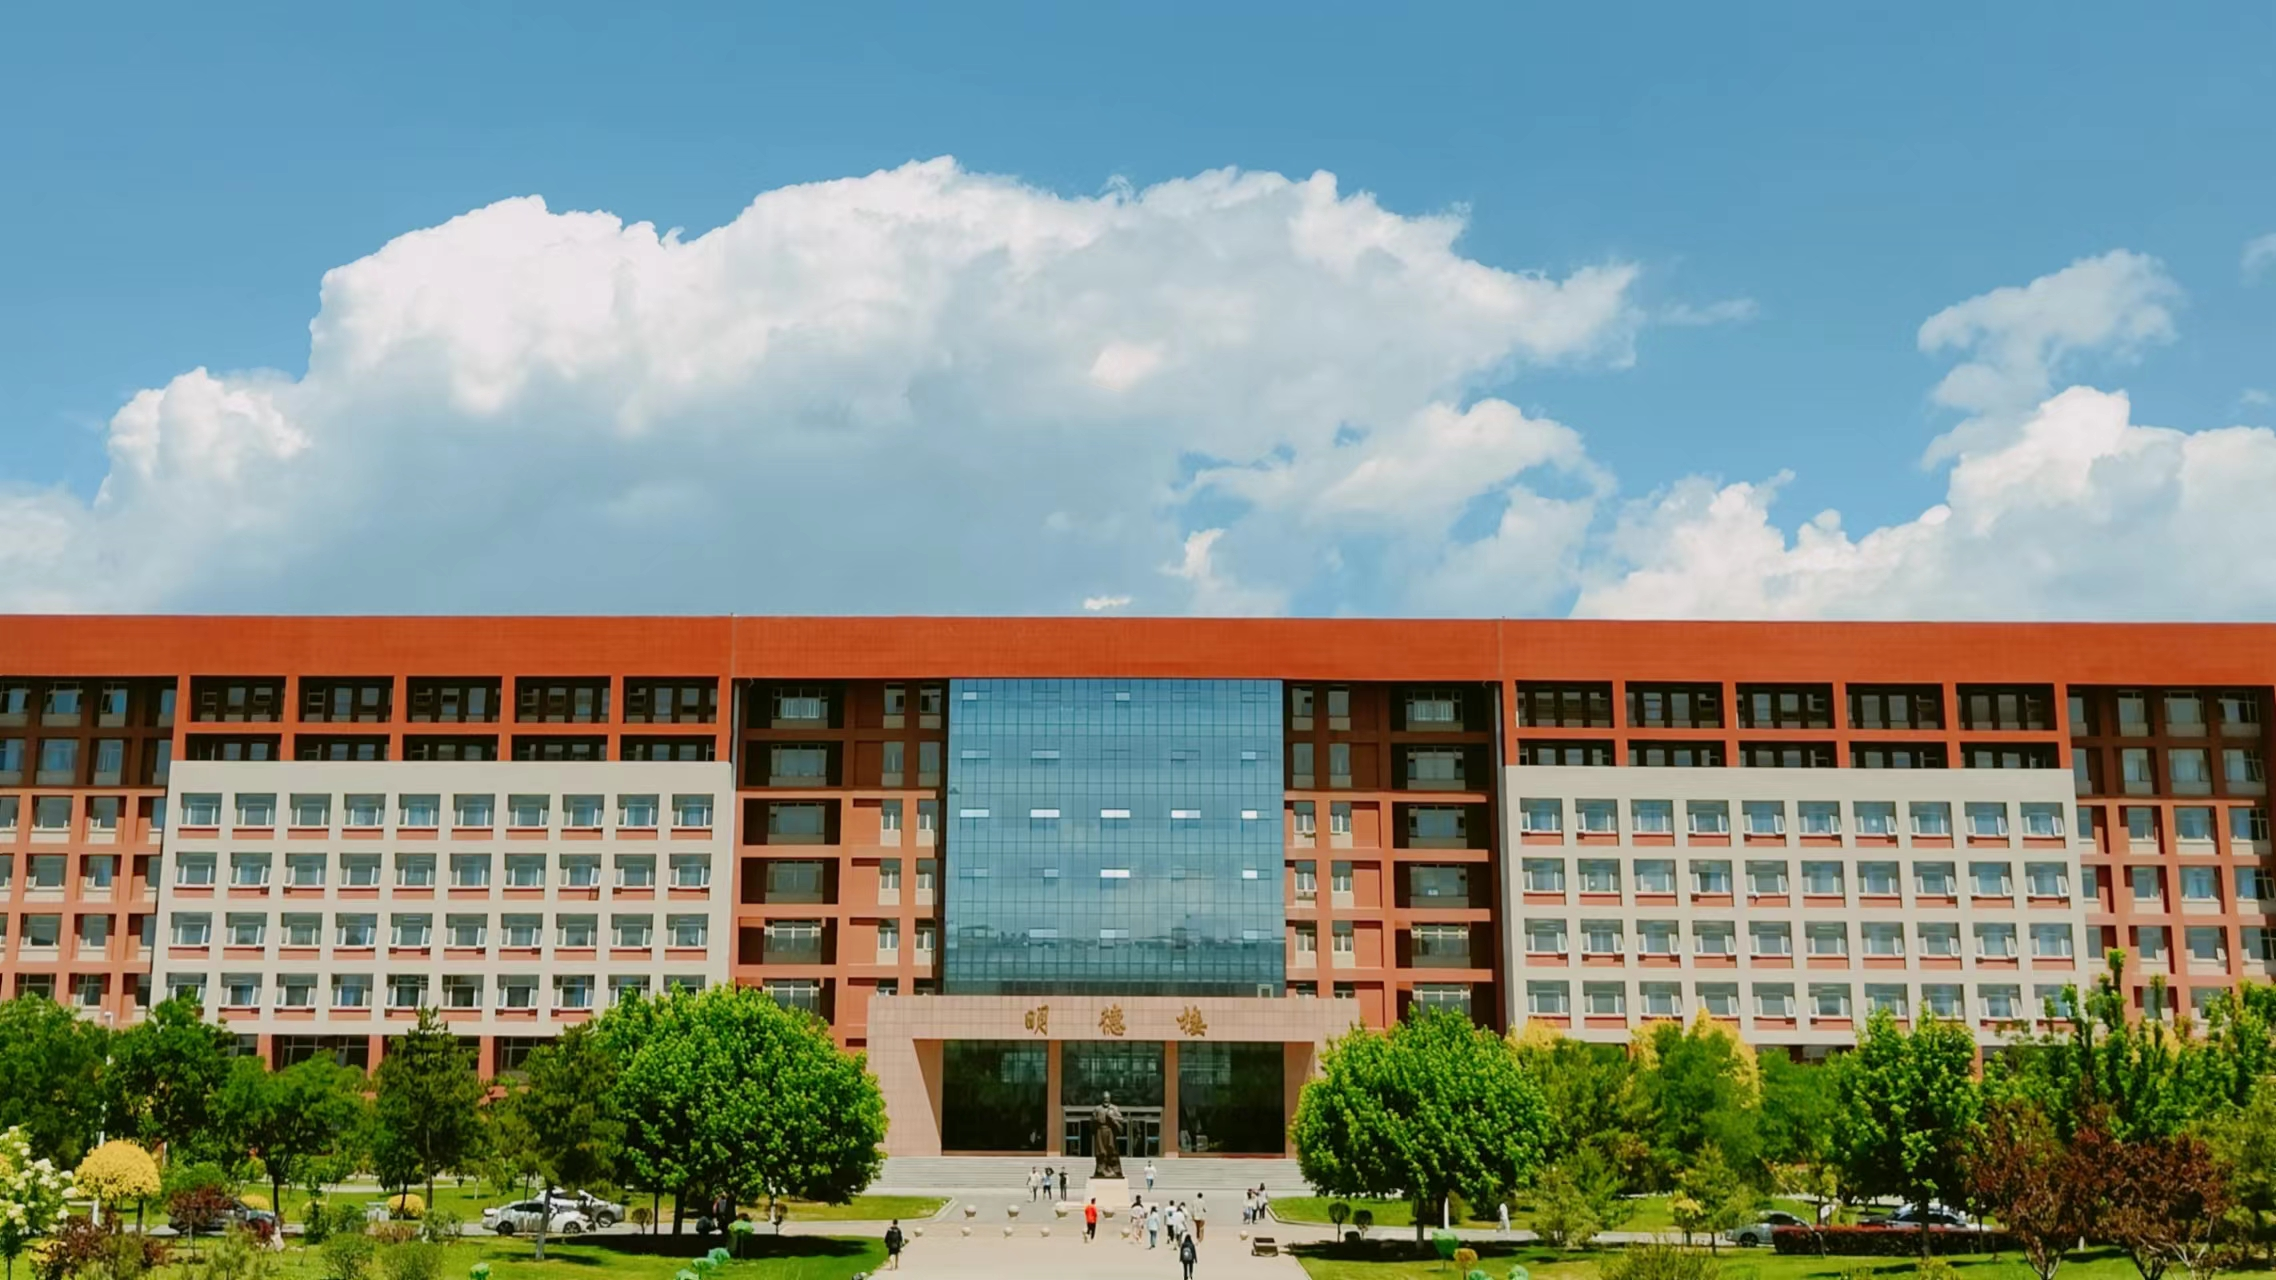
\includegraphics[width=1\textwidth]{opening.jpg}
		
		% 插入作者和日期
		\vspace{50mm}
		\headingfont\bfseries\Large\@author
	\end{center}
	\vfill
	\clearpage
}
\makeatother

% 自定义盒子
\usepackage{tcolorbox}
\usepackage{wrapfig}
\def\fullboxbegin{
	\bigskip
	\begin{tcolorbox}[colback=color1,colframe=color1,coltext=white,arc=0mm,boxrule=0pt]
	}
	\def\fullboxend{\end{tcolorbox}\medskip}
%
\def\leftboxbegin{
	\begin{wrapfigure}{l}{0.5\textwidth}
		\begin{tcolorbox}[colback=color1,colframe=color1,coltext=white,arc=0mm,boxrule=0pt]
		}
		\def\leftboxend{
		\end{tcolorbox}
	\end{wrapfigure}
}
%
\def\rightboxbegin{
	\begin{wrapfigure}{r}{0.5\textwidth}
		\begin{tcolorbox}[colback=color1,colframe=color1,coltext=white,arc=0mm,boxrule=0pt]
		}
		\def\rightboxend{
		\end{tcolorbox}
	\end{wrapfigure}
}
%
\newcounter{frames}
\def\frameboxbegin#1{
	\bigskip
	\refstepcounter{frames}
	\begin{tcolorbox}[colback=white,colframe=color1,arc=0mm,title={\MakeUppercase{\textbf{ \arabic{frames}}: #1}}]
	}
	\def\frameboxend{
	\end{tcolorbox}
}
